\chapter{Rimandi alla teoria dell'informazione}
\section{Rappresentazione matematica di oggetti}
Per parlare di Crittografia dobbiamo introdurre alcune nozioni matematiche relative alla rappresentazione di oggetti. Rappresentare matematicamente un oggetto significa attribuirgli un nome: dobbiamo fare ciò in modo rigoroso.
\paragraph{Alfabeto} Un \emph{alfabeto} è un insieme finito di caratteri detti simboli. 
\subsection{Rappresentazione degli oggetti con l'alfabeto} Un oggetto è rappresentato da una sequenza ordinata di caratteri dell'alfabeto. A oggetti diversi corrispondono sequenze diverse ed il numero di oggetti rappresentabili è infinito (fissata una lunghezza qualsiasi posso sempre creare sequenze più lunghe). 
Fissato un alfabeto $\Gamma$ tale che $|\Gamma| = s$ (dove $s$ è il numero di caratteri dell'alfabeto) e fissati \emph{N} oggetti da rappresentare otteniamo:
\begin{itemize}
	\item $d(s, N)$: è la lunghezza della sequenza più lungha di un oggetto dell'insieme
	\item $d_{min}(s, N)$: valore minimo di $d(s, N)$ tra tutte le rappresentazioni possibili
\end{itemize}
Un metodo di rappresentazione è tanto migliore tanto più $d(s, N)$ si avvicina a $d_{min}(s, N)$.

\subsubsection{Alfabeto unario}
Prendiamo un alfabeto con un solo simbolo ($s=1$): $\Gamma = \{0\}$
\paragraph{Variazione di N} L’unica possibilità che abbiamo per costruire sequenze diverse è alterare la lunghezza $N$, visto che le sequenze sono solo ripetizioni dell’unico carattere presente nell’alfabeto (0, 00, 000, …). 
\[\Longrightarrow d_{min}\left(1,N\right)=N\]
La rappresentazione non è comoda, ma soprattutto è poco efficiente.


\subsubsection{Alfabeto binario}
Passiamo a un alfabeto con due caratteri ($s = 2$). 
\[\Gamma = \{0, 1\}\]
$\forall k \geq 1$ (dove $k$ è la lunghezza della sequenza) si hanno $2^{k}$ sequenze, quindi il numero totale di sequenze lunghe da 1 a k è (data la lunghezza $k$ consideriamo anche le possibili sequenze realizzabili con un numero di caratteri minori a $k$):
$$
\sum^{k}_{i=0} 2^{i} = 2^{k+1} - 2
$$
Nel risultato finale si ha $-2$ invece di $-1$ visto che non si considera $i=0$. Per $N$ oggetti da rappresentare imponiamo che il numero di sequenze possibili sia minimo uguale ad $N$:
\begin{align*}
	2^{k+1}-2 &\geq N\\
	2^{k+1} &\geq N+2\\
	(k+1)\log(2) &\geq \log(N+2)\\
	(k+1) &\geq \frac{\log(N+2)}{\log(2)}\\
	k&\geq \log_2(N+2)-1
\end{align*}
troviamo il minimo applicando l'operatore \emph{ceil}
$$ k_{min}=d_{min}(2, N) = \lceil \log_{2}(N+2) - 1 \rceil $$
$$ \lceil \log_{2}N \rceil - 1 \leq d_{min}(2, N) \leq \lceil \log_{2}N \rceil $$

\paragraph{Esempio} Facciamo un esempio con $N=7$ (vogliamo sette sequenze di caratteri diverse), abbiamo 
$\left\lceil{\log}_2{7}\right\rceil=3$, dunque possiamo costruire N sequenze differenti tutte di lunghezza $\left\lceil{\log}_2{7}\right\rceil$
\[000,\ 001,\ 010,\ 011,\ 100,\ 101,\ 110\]La cosa è importante nelle applicazioni crittografiche: parole di pari lunghezza per evitare l’uso di separatori (cioè simboli che mi segnalano la fine di una parola e l’inizio della successiva).


\subsubsection{Alfabeto $s-$ario}
Abbiamo un alfabeto caratterizzato da $s$ caratteri. Possiamo costruire N sequenze differenti tutte di $ \lceil \log_{s}N \rceil $ caratteri.

\paragraph{Esempio}  Supponiamo di avere $\Gamma$ e di voler generare $1000$ sequenze:
\[\text{$\Gamma = \{0, \dots, 9 \}$ $\implies$ $\lceil \log_{10}1000\rceil = 3 $ cioè i numeri da 000 a 999}\]
Usare sequenze tutte della stessa lunghezza è vantaggioso perché posso concatenare più oggetti senza usare un separatore. Si dice \textbf{rappresentazione efficiente} una rappresentazione che usa un numero massimo di caratteri di ordine logaritmico nella cardinalità dell'insieme da rappresentare (N) quindi bisogna avere almeno 2 caratteri.

\subsection{Rappresentazione di interi}
La rappresentazione degli interi è una rappresentazione di tipo posizionale, dove il valore del numero dipende anche dalla posizione. Risulta efficiente  indipendentemente dalla base $s \geq 2$ scelta perché un intero $N$ costituito da $d$ cifre soddisfa la seguente condizione: \[\lceil \log_{2}N \rceil \leq d \leq \lceil \log_{2}N \rceil + 1\]
Abbiamo il concetto di \textbf{riduzione logaritmica} tra il valore di un numero N e la lunghezza della sua rappresentazione. Per avere complessità polinomiale il numero di istruzioni dell’algoritmo deve crescere come il logaritmo del valore (e non come il valore!!!).
\section{Differenza tra calcolabilità e complessità}
A questo punto possiamo distinguere la teoria della calcolabilità da quella della complessità:
\begin{itemize}
	\item \textbf{Teoria della calcolabilità}\\La teoria della calcolabilità studia gli algoritmi da un punto di vista di risoluzione algoritmica: quali problemi possono essere risolti algoritmicamente in un calcolatore (problemi decidibili) e quali no (problemi non decidibili).
	\item \textbf{Teoria della complessità}\\La teoria della complessità studia gli algoritmi (problemi decidibili) da un punto di vista dell’efficienza (problema efficiente, complessità polinomiale, o problema intrattabile, complessità esponenziale)
\end{itemize}

\section{Teoria della calcolabilità}
La calcolabilità si occupa della potenza e dei limiti dei sistemi di calcolo. La disciplina ha un secolo di vita, nasce quando i logici matematici iniziano ad esplorare i concetti di computazione, algoritmo e risoluzione algoritmica di problemi. 
\subsection{Problemi computazionali}
I problemi a cui siamo interessati sono problemi computazionali, che hanno una formulazione matematica precisa e una risoluzione algoritmica. Si distinguono in:
\begin{itemize}
	\item \textbf{problemi non decidibili}, non risolvibili algoritmicamente in un calcolatore (ne è stata dimostrata l’esistenza prima della nascita del calcolatore);
	\item \textbf{problemi decidibili}, che ammettono una soluzione algoritmica. Se consideriamo la complessità distinguiamo questi problemi in
	\begin{itemize}
		\item \textbf{problemi trattabili} (algoritmi di costo polinomiale, esistono algoritmi di complessità polinomiale che ne permettono la risoluzione),
		\item \textbf{problemi intrattabili} (algoritmi di costo esponenziale, non solo non esistono algoritmi di complessità polinomiale, ma si è anche dimostrata l'esistenza di un limite inferiore),
		\item \textbf{problemi aventi stato computazionale non noto} (non esistono algoritmi di complessità polinomiale, ma non si è dimostrata l'esistenza di un limite inferiore - dunque potrebbero essere scoperti in futuro algoritmi aventi minore complessità).
	\end{itemize}
\end{itemize}


%\subsection{Insieme dei problemi trattabili}
%Tra i problemi decidibili abbiamo i problemi trattabili, ossia problemi risolvibili con algoritmi di complessità polinomiale:
%\begin{itemize}
%	\item	ricerca di chiavi in array, liste, alberi (algoritmo di ricerca lineare, ma anche algoritmo di ricerca binaria – più efficiente);
%	\item	problemi sui grafi, si pensi ad esempio alla ricerca di un ciclo Euleriano.
%\end{itemize}
%Per quanto riguarda i problemi non risolvibili con complessità polinomiale (sempre tra i problemi decidibili) si distinguono le due classi successive.

%\subsection{Insieme dei problemi intrattabili}
%I problemi intrattabili richiedono obbligatoriamente algoritmi di complessità esponenziale: presentano un limite inferiore (ripensare a quanto visto ad algoritmi), dunque non è possibile individuare algoritmi con complessità inferiore. Gli esempi classici sono:
%\begin{itemize}
%	\item generazione delle sequenze binarie e delle permutazioni (il numero di sequenze è esponenziale in numero, non posso impiegare un tempo minore);
%	\item torre di Hanoi (spostamento dei dischi dal primo al terzo piolo tenendo conto di alcune regole).
%\end{itemize}

%\subsection{Insieme dei problemi aventi stato computazionale non noto}
%Ci sono problemi il cui stato computazionale non è noto, per esempio la ricerca del cammino hamiltoniano. Sappiamo risolvere questi problemi (sono problemi decisionali) con algoritmi di complessità esponenziale, ma contrariamente a prima non abbiamo un limite inferiore: nessuno ha dimostrato in modo rigoroso che non esistono problemi di complessità inferiore. 


\subsection{Esistenza di problemi non decidibili}
Vogliamo dimostrare l'esistenza di problemi non decidibili.
\subsubsection{Definizione: insiemi con stessa cardinalità}
Due insiemi $A$ e $B$ hanno la stessa cardinalità 
\[|A|=|B|\]
\emph{se e solo se} si può stabilire una corrispondenza biunivoca tra i loro elementi (una mappa)\footnote{Rinfreschiamoci la memoria sulla biunivocità grazie a Wikipedia: in matematica una corrispondenza biunivoca tra due insiemi X e Y è una relazione binaria tra X e Y, tale che ad ogni elemento di X corrisponda uno ed un solo elemento di Y, e viceversa ad ogni elemento di Y corrisponda uno ed un solo elemento di X. In particolare, la corrispondenza biunivoca è una relazione di equivalenza.}.
\subsubsection{Definizione: insieme numerabile} Un insieme è \emph{numerabile} (ha una infinità numerabile di elementi) \emph{se e solo se} i suoi elementi si possono mettere in corrispondenza biunivoca con i numeri naturali.
\begin{itemize}
	\item Un insieme numerabile può essere elencato: \[a_1, a_2, \dots, a_n, \dots\]
	\item Le stringhe di lunghezza finita di simboli di un alfabeto finito sono un insieme numerabile
	\begin{itemize}
		\item Il numero di queste stringhe è infinito, ma la cosa importante è che \textbf{ogni sequenza dell’elenco abbia una distanza finita dall’inizio} (cioè deve essere possibile raggiungere qualsiasi sequenza attraverso un numero finito di passi dalla prima sequenza).
		
		\item Usiamo l'\emph{ordinamento canonico}:
		\begin{itemize}
			\item si ordinano le sequenze per lunghezza crescente
			\item le sequenze di pari lunghezza si ordinano alfabeticamente (supponendo di avere creato una regola di ordine tra i caratteri)
		\end{itemize}
		
		Quindi una sequenza $s$ arbitraria si troverà tra quelle $|s|$, posizione alfabetica tra queste.
		
		\item \textbf{Esempio}.
		\begin{align*}
			&\Gamma=\{a,b,c,\dots,z\}\\
			&a,b,c,\dots,z\\
			&aa,ab,\dots,az,ba,\dots,bz,\dots,za,\dots,zz\\
			&aaa,aab,\dots,baa,\dots,zaa,\dots,zzz\\
			&aaaa,\dots
		\end{align*}		
		Seguendo questo metodo ogni sequenza corrisponde ad un numero $\in \mathbb{N}$ ed ogni naturale ha una sequenza associata.
		\item \textbf{Attenzione}. Questo si può fare perché abbiamo preso sequenze di lunghezza finita, per sequenze di lunghezza infinita non esiste una enumerazione.
	\end{itemize} 
	\item \textbf{Esempi di insiemi non numerabili}.
	\begin{itemize}
		\item $\mathbb{R}$ e sottoinsiemi (per esempio $\mathbb{R}$ ristretto a $(0, 1)$ o $[0, 1]$)
		\item \underline{\textbf{insieme delle funzioni in una o più variabili}}
	\end{itemize}
\end{itemize}



\subsubsection{Dimostrazione} Dimostriamo per quanto riguarda l'ultimo insieme citato tra i non numerabili. 
\begin{itemize}
	\item Un problema computazionale può essere visto come una funzione matematica che associa ad ogni insieme di dati su $k$ numeri interi il risultato su $j$ numeri interi:
	$$ f :  \mathbb{N}^{k} \longrightarrow \mathbb{N}^{j} $$
	Se siamo in grado di dimostrare che questo insieme di funzioni non è numerabile allora possiamo dire la stessa per l’insieme di problemi computazionali.
	\item Per semplificarci la vita dimostriamo la cosa su un sottoinsieme
	\[F = \{f | f: \mathbb{N} \longrightarrow \{0, 1\}\}\]
	Ogni $f \in F$ può essere rappresentata da una sequenza infinita:
	\begin{table}[!h]
		\centering
		\begin{tabular}{c|c|c|c|c|c|c|c}
			$x$ & 0 & 1 & 2 & 3 & \_ & n & \_  \\
			\hline
			$f(x)$ & 0 & 1 & 0 & 1 & \_ & 0 & \_
		\end{tabular}
	\end{table}
	
	oppure da una regola finita di costruzione:
	
	\[f(x) =
	\begin{cases}
		$0 \text{se x è pari}$ \\
		$1 \text{se x è dispari}$
	\end{cases}\]
	\item Supponiamo per assurdo che $F$ sia numerabile, quindi è possibile trovare una enumerazione per $f \in F$: questo significa poter associare un numero progressivo nella numerazione e costruire una tabella avente un numero infinito di righe (possibili funzioni) e colonne (possibili valori in ingresso).
	\begin{table}[!h]
		\centering
		\begin{tabular}{c|c c c c}
			$x$ & 0 & 1 & 2 & \_  \\
			\hline
			$f_0(x)$ & 1 & 0 & 1 & \_ \\ 
			$f_1(x)$ & 0 & 0 & 1 & \_ \\ 
			$f_2(x)$ & 1 & 1 & 0 & \_ \\ 
		\end{tabular}
	\end{table}
	\item Per dimostrare la non numerabilità dell'insieme mi basta individuare una sola funzione non numerabile. Consideriamo dunque la seguente funzione:
	
	\[g(x) = 
	\begin{cases}
		$0 \text{ se }$ f_x(x) = 1 \\
		$1 \text{ se }$ f_x(x) = 0 \\
	\end{cases}\]
	$g \in F$ perché è una funzione dai naturali a \{0, 1\} ma non può corrispondere a nessuna delle funzioni nella tabella precedente:
	\begin{itemize}
		\item non può essere $f_0$ in quanto differisce in $x = 0$
		\item non può essere $f_1$ in quanto differisce in $x = 1$
		\item e così via $\forall n$
	\end{itemize}
	\item Diciamo la cosa in modo più formale:
	\begin{itemize}
		\item Supponiamo per assurdo che esista un valore $i$ tale che $f_i \equiv g$.
		\item Possiamo dire che $f_i\equiv g$, tuttavia per definizione
		\[g(j)=\begin{cases}0&f_j(j)=1\\1&f_j(j)=0\end{cases}\]
		Quanto scritto consiste di fatto nella funzione di complementazione, quindi per forza ho $g\left(j\right)\neq f_j\left(j\right)$. Noi abbiamo considerato la diagonale, ma nulla ci vieta di considerare linee arbitrarie che attraversano la tabella toccando tutte le righe e tutte le colonne esattamente una volta.
		\item Per qualunque numerazione scelta esiste sempre almeno una funzione esclusa, dunque ${F}$ non è numerabile.
		\item Se $F$ è un insieme non numerabile allora tutti gli insiemi che lo contengono non sono numerabili:
		\begin{itemize}
			\item $f:\mathbb{N} \to \mathbb{N}$
			\item $f:\mathbb{N} \to \mathbb{R}$
			\item $f:\mathbb{R} \to \mathbb{R}$
			\item $f:\mathbb{N}^k\to \mathbb{N}^j$ (insieme delle funzioni in una o più variabili)
		\end{itemize}
		\textbf{L'insieme dei problemi computazionali non è numerabile}!
	\end{itemize}
\end{itemize}

\subsubsection{Conclusioni: il problema della rappresentazione}
L'informatica rappresenta tutte le sue entità in forma digitale come "sequenze finite di simboli di alfabeti finiti". Possiamo dire quindi che la conoscenza umana è numerabile. L'algoritmo è una sequenza finita di operazioni, completamente e univocamente determinate. La formulazione di un algoritmo dipende dal modello di calcolo utilizzato: se uso la macchina di Turing ho una codifica, se uso il C ne ho un'altra, ecc. Qualsiasi codifica si scelga gli algoritmi sono sempre descritti da una sequenza finita di caratteri di un alfabeto finito. 

\paragraph{In conclusione}
\begin{itemize}
	\item L'insieme degli algoritmi è infinito ma numerabile.
	\item \underline{I problemi computazionali sono infiniti ma non numerabili}.
\end{itemize}
Se l'insieme dei problemi computazionali non è numerabile allora non è possibile stabilire una corrispondenza biunivoca tra insieme dei problemi computazionali e quello degli algoritmi, ergo \textbf{esistono problemi computazionali non associati a un corrispondente algoritmo di calcolo} (ricordare quanto detto all'inizio su due insiemi che hanno la stessa cardinalità).

$\hfill\blacksquare$

\subsection{Problema dell'arresto (Halt problem) e sua indecidibilità}
Il problema dell’arresto è un problema indecidibile, individuato da Alan Turing nel 1930. 
\begin{itemize}
	\item Presi ad arbitrio un algoritmo A e i suoi dati di input d, dobbiamo decidere in tempo finito (volendo anche esponenziale, basta che sia finito) se la computazione di A su d termina (il programma termina la sua esecuzione) o non termina (va in loop, cioè continua a ripetere la stessa sequenza di istruzioni all’infinito ).
	\item In sostanza vogliamo individuare \textbf{un algoritmo che indaga sulle proprietà di un altro algoritmo}, cioè un algoritmo che ha come input un altro algoritmo. 
	\begin{itemize}
		\item Un algoritmo A, comunque formulato, può operare sulla rappresentazione di un altro algoritmo B. Poniamo quindi A(B).
		\item Possiamo fare anche A(A), per esempio se l’algoritmo A deve calcolare la lunghezza del file che rappresenta l’algoritmo.
	\end{itemize}
\end{itemize}
\paragraph{Dimostrazione di Turing sull'indecibilità del problema}
\begin{itemize} 
	\item Anche questa volta ragioniamo per assurdo: supponiamo che esista un algoritmo ARRESTO che prende A e d come input, e determina la risposta in tempo finito. In particolare
	\[\text{ARRESTO}(A,d)=\begin{cases}1&A(d)\text{ termina}\\0&A(d)\text{ non termina}\end{cases}\]
	Risulta scontato che l’algoritmo non deve consistere nell’eseguire il programma: questo perché se il problema non si arresta allora la funzione non può restituire 0 in tempo finito.
	\item Immaginiamo $D=A$, quindi $A(A)$ (algoritmo che ha come input se stesso). Possiamo dire
	\[\text{ARRESTO}\left(A,A\right)=1\Longrightarrow A\left(A\right)\mathrm{\ termina}\]
	fin qui nulla di strano.
	\item Se esiste l’algoritmo ARRESTO allora esiste il seguente algoritmo PARADOSSO:
	\begin{verbatim}
		PARADOSSO(A): while(ARRESTO(A,A)) { }
	\end{verbatim}
	la condizione nel while è true e non viene influenzata dal corpo (non cambia).
	\item L'algoritmo $\text{PARADOSSO}(A)$ non termina se l'algoritmo $A(A)$ termina, cioè se abbiamo $\text{ARRESTO}\left(A,A\right)=1$. Posso dire che $\text{PARADOSSO}(A)$ termina solo se $A(A)$ non termina.
	\[\text{PARADOSSO}\left(A\right)\mathrm{ termina}\Longleftrightarrow x=\text{ARRESTO}\left(A,A\right)=0\]
	\item Consideriamo $\text{PARADOSSO}(\text{PARADOSSO})$: osservo che termina solo se 
	\[\text{PARADOSSO}\left(\text{PARADOSSO}\right)\mathrm{termina}\Longleftrightarrow x=\text{ARRESTO}\left(\text{PARADOSSO},\ \text{PARADOSSO}\right)=0\]
	Ecco la contraddizione: stiamo dicendo che $\text{PARADOSSO}\left(\text{PARADOSSO}\right)$ termina solo se $\text{PARADOSSO}\left(\text{PARADOSSO}\right)$ non termina. La contraddizione può essere risolta solo affermando la non esistenza di PARADOSSO, dunque non può esistere nemmeno ARRESTO.
\end{itemize}
$\hfill\blacksquare$

\noindent Un algoritmo ARRESTO sarebbe uno strumento estremamente potente: permetterebbe, ad esempio, di dimostrare congetture ancora aperte sugli interi (esempio: la congettura di Goldbach\footnote{Da Wikipedia. In matematica, la congettura di Goldbach è uno dei più vecchi problemi irrisolti nella teoria dei numeri. Essa afferma che ogni numero pari maggiore di 2 può essere scritto come somma di due numeri primi (che possono essere anche uguali).}).


\subsection{Problema indecidibile: equivalenza tra programmi}
\[\boxed{\text{E' indecidibile stabilire l'equivalente tra due programmi (stesso input $\implies$ stesso output)}}\]
Turing afferma che non esistono algoritmi che decidono il comportamento di altri algoritmi esaminandoli dall’esterno, cioè senza passare dalla loro simulazione.

\subsection{Modelli di Calcolo e complessità (tesi di Churc-Turing)}
Poniamoci una domanda
\[\text{\underline{La decidibilità dipende dal modello di calcolo o è una caratteristica del problema?}}\]
La domanda può essere posta in altri modi:
\begin{itemize}
	\item i linguaggi di programmazione esistenti sono tutti equivalenti? 
	\item esistono linguaggi più potenti e/o più semplici di altri? 
	\item ci sono algoritmi descrivibili in un linguaggio, ma non in un altro? 
	\item è possibile che problemi attualmente irrisolvibili possano essere risolti in futuro con altri linguaggi o con altri calcolatori?
\end{itemize}
Non abbiamo un teorema che ci permetta di rispondere in modo univoco alle domande precedenti, ma abbiamo una tesi secondo cui il modello di calcolo non influisce sulla decidibilità (tesi di Churc-Turing): \textbf{tutti i ragionevoli modelli di calcolo risolvono esattamente la stessa classe di problemi}. 
\paragraph{Significato} Questo significa che i modelli di calcolo si equivalgono nella possibilità di risolvere problemi (anche se con diversa efficienza), quindi incrementi qualitativi alla struttura di una macchina (anche al computer quantistico ), o alle istruzioni di un linguaggio di programmazione, servono solo a:
\begin{itemize}
	\item abbassare il tempo di esecuzione;
	\item rendere più agevole la programmazione.
\end{itemize}

\subsection{Algoritmi polinomiali ed esponenziali a confronto}
Perché si pone questa demarcazione netta tra algoritmi di costi polinomiale e algoritmi di costo esponenziale? 
Supponiamo di avere un calcolatore $C_1$ e un calcolatore $C_2$, entrambi hanno a disposizione un tempo t e devono risolvere lo stesso problema (per cui abbiamo lo stesso algoritmo risolutivo). Vogliamo vedere come cambia la dimensione dei dati trattabili a parità di tempo, in macchine con capacità computazionali diverse. Quindi:
\begin{itemize}
	\item $n_1$ sono i dati trattabili nel tempo $t$ su $C_1$, $n_2$ sono i dati trattabili nel tempo $t$ su $C_2$
	\item Usare $C_2$ per un tempo $t$ equivale a usare $C_1$ per un tempo $k\ \cdot t$
\end{itemize}
\begin{center}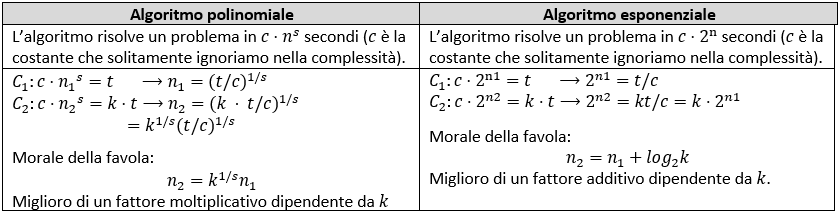
\includegraphics[scale=.9]{images/1.PNG}\end{center}
Si osserva che il miglioramento dell’algoritmo esponenziale è minore rispetto al miglioramento dell’algoritmo polinomiale. 
L’algoritmo efficiente è molto più importante della piattaforma hardware usata: 
\[\boxed{\text{Un algoritmo inefficiente lo è su qualunque piattaforma.}}\]

\section{Premessa alla teoria della complessità}
Per capire quanto è efficiente un algoritmo è necessario chiarire i parametri su cui valutare l'efficienza. Solitamente si prende a riferimento il tempo di esecuzione oppure l'occupazione di memoria. In entrambi i casi si descrive l'andamento attraverso una funzione matematica.
\begin{itemize}
	\item Successivamente dobbiamo determinare la variabile indipendente su cui si lavora: solitamente si prende il parametro $n$, che è la dimensione dell'ingresso (o dimensione dei dati). Il parametro indica la lunghezza della sequenza che specifica il valore dei dati per una particolare istanza del problema.
	\item Consideriamo la seguente funzione per la moltiplicazione
	\begin{verbatim}Molt(a,b)\end{verbatim}
	Supponiamo di avere i numeri $a=351, b=66$. Possiamo porre $n=5$ poichè le cifre tra i due numeri sono cinque. A questo punto sorge il problema che il numero di cifre dipende dalla base di rappresentazione adottata. Come risolviamo? Ripensiamo a quanto visto per la rappresentazione di oggetti attraverso sequenze finite costituite da caratteri di un alfabeto finito: per costruire $N$ sequenze differenti ho bisogno del seguente numero di caratteri
	\[\lceil \log_n N \rceil\]
	dove $n$ è il numero di caratteri dell'alfabeto. Il numero di caratteri dell'alfabeto è letteralmente la base (la base $n$ è costituita da $n$ cifre che vanno da $0$ ad $n-1$). Sappiamo che è possibile fare un cambio di base nel logaritmo con la seguente formula
	\[\log_c a = \frac{\log_b a}{\log_b c} \longrightarrow \left(\log_c a\right) \left(\log_b c\right) = \log_b a\]
	Questo significa che nel passaggio da una base a un'altra si va a moltiplicare per un fattore costante. Si consideri per esempio un intero: esso è rappresentato in base $10$ col seguente numero di cifre
	\[\lceil \log_{10}N \rceil\]
	Per passare dalla base $10$ alla base $2$ andrò a moltiplicare il numero di cifre per $\log_2 10$. Da questo deduciamo la necessità di ragionare per \textbf{ordini di grandezza}.
	\item L'ordine di grandezza è un insieme infinito che comprende tutte le funzioni che hanno un particolare comportamento rispetto a una funzione $g(n)$. Esse sono:
	\begin{itemize}
		\item $O(g(n))$, l'insieme di tutte le funzioni $f(n)$ per cui esistono due costanti positive $c,n_0$ tali che 
		$$f(n) \leq c g(n)$$
		questo $\forall n \geq n_0$. Al crescere di $n$ il comportamento della funzione $f(n)$ è limitato \textbf{\underline{superiormente}} dalla funzione $g(n)$
		\item $\Omega(g(n))$, l'insieme di tutte le funzioni $f(n)$ per cui esistono due costanti positive $c,n_0$ tali che 
		$$f(n) \geq c g(n)$$
		questo $\forall n \geq n_0$. Al crescere di $n$ il comportamento della funzione $f(n)$ è limitato \textbf{\underline{inferiormente}} dalla funzione $g(n)$
		\item $\Theta(n)$, l'insieme di tutte le funzioni $f(n)$ per cui esistono due costanti positive $c,n_0$ tali che
		$$c_1 g(n) \leq f(n) \leq c_2 g(n)$$
		questo $\forall n \geq n_0$. Al crescere di $n$ il comportamento della funzione $f(n)$ è limitato \textbf{\underline{superiormente}} e \textbf{\underline{inferiormente}} dalla funzione $g(n)$. Segue
		$$f(n)=\Theta(g(n)) \Longrightarrow f(n)=O(g(n)) \text{ e } f(n)=\Omega(g(n))$$
	\end{itemize}
\end{itemize}

\section{Teoria della complessità}
Possiamo immaginare un problema $\Pi$ come una funzione matematica $f: I \to S$, dove:
\begin{itemize}
	\item $I$: insieme delle \emph{istanze} di ingresso
	\item $S$: insieme delle \emph{soluzioni}
\end{itemize}
\subsection{Tipologie di problemi}
Alcune tipologie di problemi sono:
\begin{itemize}
	\item \textbf{Problemi decisionali}\\ Problemi dove l'insieme delle soluzioni è un insieme binario $S = \{0, 1\}$. 
	\begin{itemize}
		\item Un'istanza $x \in I$ è detta istanza positiva o accettabile se $\Pi(x) = 1$ 
		\item Un'istanza $x \in I$ è detta istanza negativa se: $\Pi(x) = 0$
		\item \textbf{Esempi}: numero primo, grafo connesso...
	\end{itemize}
	\item \textbf{Problemi di ricerca}\\Data un'istanza $x \in I$ vogliamo trovare una soluzione $s$ (trovare un cammino tra due vertici, ecc)
	\item \textbf{Problemi di ottimizzazione}\\Data un'istanza $x \in I$ si vuole trovare la migliore soluzione $s$ tra tutte quelle ammissibili (cammino minimo, ecc)
\end{itemize}
\subsection{Ruolo di problemi decisionali e di ottimizzazione nella teoria}
La teoria della complessità fa riferimento alla sola classe decisionale in quanto:
\begin{itemize}
	\item essendo $s = \{0, 1\}$ non ci si deve preoccupare del tempo per restituire la soluzione (influisce solo il tempo per il calcolo della soluzione);
	\item la difficoltà è già presente nella sua versione decisionale.
\end{itemize} 
Molti problemi di interesse pratico sono problemi di ottimizzazione. Possiamo esprimere i problemi di ottimizzazione in forma decisionale.
\paragraph{Esempio}
\begin{itemize}
	\item MAX-CLIQUE: trovare la clique più grande in un grafo G
	\item CLIQUE decisionale: esiste una clique in G di almeno k vertici? 	
\end{itemize}
CLIQUE decisionale non è più difficile di MAX-CLIQUE. Supponiamo di saper risolvere MAX-CLIQUE: se io so trovare la risposta allora automaticamente trovo risposta alla versione decisionale del problema.  Il problema di ottimizzazione è almeno tanto difficile quanto il corrispondente problema decisionale. Lo studio del problema decisionale permette di fornire un limite inferiore alla versione di ottimizzazione.

\subsection{Teoria della verifica}
\subsubsection{Concetto di \emph{certificato}}
In un problema decisionale siamo interessati a verificare se un'istanza del problema soddisfa una certa proprietà. In alcuni problemi è possibile fornire un certificato per ogni istanza accettabile, che ci convinca della sua accettabilità. Questo significa che non siamo tanto interessati alla soluzione nello specifico, ma a un qualcosa che attesti la sua esistenza.

\paragraph{Definizione} Si definisce il \textbf{certificato} come un attestato "breve" di esistenza di una soluzione con determinate proprietà (una descrizione succinta della soluzione), si definisce solo per le istanze accettabili (gli attestati di non esistenza non sono facili da costruire).

\subsubsection{Verifica in tempo polinomiale}
Nella teoria della verifica utilizziamo il costo della verifica di un certificato per una istanza positiva per caratterizzare la complessità del problema stesso. \paragraph{Definizione} Un problema $\Pi$ è \textbf{verificabile in tempo polinomiale} se
\begin{itemize}
	\item ogni istanza accettabile $x$ di $\Pi$ di lunghezza $n$ ammette un certificato $y$ di lunghezza polinomiale in $n$
	\item esiste un algoritmo di verifica polinomiale in $n$ ed applicabile ad ogni coppia \\$<x$, $y>$ che attesta se $x$ è accettabile.
\end{itemize}
\paragraph{Utilità della teoria della verifica ($\Pi \in NP$?)}  Quanto è effettivamente utile la teoria della verifica? Il dubbio può venire visto che il certificato è un qualcosa di molto vicino alla soluzione. La teoria della verifica ci aiuta a costruire una gerarchia di complessità dei problemi (cioè capire quanto un problema è facile o difficile), ma non aiuta nella risoluzione dei problemi stessi.
\begin{itemize}
	\item Chi ha una soluzione può verificare in tempo polinomiale se l’istanza è veramente accettabile (classe NP).
	\item Chi non ha una soluzione non ha il certificato e deve individuarlo. Lo faccio con metodo forza bruta: in tempo esponenziale considero tutti i casi possibili. 
\end{itemize}
Abbiamo introdotto la teoria della verifica per affrontare, poco più avanti, le classi NP ed NP-completo.

\subsection{Classi di complessità}
Dato $\Pi$ decisionale ed A algoritmo diciamo che A risolve $\Pi$ se, dato l'input $x$:
$$ A(x) = 1 \Longleftrightarrow \Pi(x) = 1 $$
Diciamo poi che A risolve $\Pi$ in tempo $t(n)$ ed in spazio $s(n)$ se il tempo di esecuzione e l'occupazione di memoria di A hanno andamento simile alle funzioni $t(n)$ e $s(n)$. Dato $f(n)$ diremo:
\begin{itemize}
	\item $\mathbf{Time(f(n))}$ \\
	Insieme dei problemi decisionali che possono essere risolti in tempo $O(f(n))$
	\item $\mathbf{Space(f(n))}$\\
	Insieme dei problemi decisionali che possono essere risolti in spazio $O(f(n))$
	\item \textbf{Classe P}.\\E' la classe di problemi che possono essere risolti in \textbf{\underline{AL PIU'}} tempo polinomiale nella dimensione dell'istanza di input.
	\begin{itemize}
		\item \textbf{Algoritmo polinomiale (tempo)}.
		Date due costanti $c,n_0>0$ tale che il numero di passi elementari è al più $n^c$ per ogni input di dimensione $n$ e per ogni $n>n_0$.
	\end{itemize}
	
	\item \textbf{Classe PSPACE}.\\
	Equivalente della classe P nello spazio. E' la classe di problemi che possono essere risolti in spazio polinomiale nella dimensione dell'istanza di input. 
	
	\item \textbf{Classe RP}.\\La classe di problemi \emph{Random-Polinomial} contiene tutti i problemi che ammettono un algoritmo di costo polinomiale randomizzato. Il test di primalità appartiene a questa classe.
	$$\boxed{P \subseteq RP \subseteq NP} $$
	
	\item \textbf{Classe EXP-TIME}\\
	La classe Exp(time) è la classe dei problemi risolvibili in  \textbf{\underline{AL PIU'}} tempo esponenziale nella dimensione $n$ dell'istanza di input.
	\[P\subseteq PSpace \subseteq Exp-Time\]
	
	NB: $P \subseteq PSpace$ perché un algoritmo polinomiale può accedere al più ad un numero polinomiale di locazioni di memoria (altrimenti dovrebbe essere esponenziale).
	
	NB: $PSpace \subseteq Exp-Time$ (abbiamo detto \textbf{\underline{AL PIU'}}, nota bene)
	
	Ad oggi non sappiamo se sono inclusioni proprie, l'unica separazione dimostrata è \[P \subset Exp-Time\] poiché abbiamo problemi risolti in $Exp$ e non in $P$ (ad esempio Hanoi)

	\item \textbf{Classe NP}\\
	NP è la classe dei problemi decisionali verificabili in tempo polinomiale.
	
	NB: NP sta per \emph{polinomiale su macchine non deterministiche}
	
	Abbiamo quindi che se si ha una soluzione essa è facile da verificare ma se non si ha una soluzione la si cerca in tempo esponenziale.
	
	NB: $P \subseteq NP$ certamente perché qualsiasi problema in P può essere risolto in tempo polinomiale. Non sappiamo però se $P \subset NP$ o $P = NP$. Per il momento la congettura pone $P \neq NP$
	\begin{center}
		
\includegraphics{images/2.PNG}
	\end{center}
	Si prenda ad esempio la SAT (lo vediamo nel dettaglio poco più avanti): è facile capire se dei valori soddisfano una formula logica, ma non è altrettanto facile individuare dei valori che soddisfano la formula logica stessa (forza brutta, analizzo tutte le possibili combinazioni).
	
	\item \textbf{Problemi NP-completi}\\
	I ricercatori, per cercare di rispondere al dilemma di P ed NP, hanno individuato all’interno della classe NP i problemi più difficili: la classe NP-completo.
	
	\underline{Questi problemi hanno una caratteristica comune}: se esistesse un algoritmo polinomiale per risolvere uno solo di questi problemi, allora tutti i problemi in NP potrebbero essere risolti in tempo polinomiale.
	
	La definizione è posta poco più avanti, a seguito della riduzione del concetto di \emph{riduzione polinomiale}.
\end{itemize}


\subsection{Riduzioni polinomiali}
Presi i problemi decisionali $\Pi_{1}$ e $\Pi_{2}$, con insiemi di input $I_{1}$ e $I_{2}$ (rispettivamente di $\Pi_{1}$ e di $\Pi_{2}$), diremo che il problema $\Pi_{1}$ si riduce in tempo polinomiale al problema $\Pi_{2}$ se esiste una funzione che mi trasforma una istanza del primo problema in una istanza del secondo problema $$f:I_{1} \to I_{2}$$
Essa è calcolabile in tempo polinomiale. Rappresentiamo la cosa con la seguente notazione:
$$ \Pi_{1} \leq_{p} \Pi_{2} $$
inoltre $$\boxed{x \text{ è accettabile per } \Pi_{1} \Longleftrightarrow f(x) \text{ è accettabile per } \Pi_{2}, \forall x \in \Pi}$$

\paragraph{Utilità} La riduzione polinomiale è utile perché supponendo di risolvere $\Pi_{2}$ in tempo polinomiale allora $\Pi_{1}$ viene tradotto in tempo polinomiale in $\Pi_{2}$ e quindi anche $\Pi_{1}$ è polinomiale:
$$ \Pi_{1} \leq_{p} \Pi_{2} \text{ e } \Pi_{2} \in P \Longrightarrow \Pi_{1} \in P $$
\subsection{Problema NP-arduo}
Un problema (non per forza decisionale) $\Pi$ si dice NP-arduo se ogni problema $\Pi' \in NP$ può essere risolto utilizzando $\Pi$ (riduco polinomialmente il problema $\Pi'$ al problema $\Pi$):
$$ \forall \Pi' \in \text{NP} \text{  } \Pi' \leq_{p} \Pi $$

\subsection{Problema NP-completo}
Un problema decisionale $\Pi$ si dice NP-Completo se
\begin{itemize}
	\item $\Pi \in \text{NP}$
	\item $\Pi$ è NP-arduo
\end{itemize} 
 Dimostriamo che se troviamo $\Pi$ NP-Completo, ma $\Pi \in P$ allora $\text{P}=\text{NP}$:
 \begin{itemize}
 	\item per ogni $\Pi' \in \text{NP}$ si ha $\Pi' \leq_p \Pi$, quindi trasformo $I_{\Pi'}$ in $I_{\Pi}$.
 	\item $I_{\Pi}$ è risolubile in tempo polinomiale, quindi qualunque $\Pi' \in \text{NP}$ è risolto in tempo polinomiale.
 \end{itemize}
$\hfill\blacksquare$

\subsection{Dimostrare che un problema è NP-arduo o NP-completo} Abbiamo visto che dimostrare $\Pi \in NP$ è semplice: basta esibire un certificato polinomiale (teoria della verifica). Non è semplice invece dimostrare che un problema è NP-arduo o NP-completo perché:
\begin{itemize}
	\item devo dimostrare che tutti i problemi NP si riducono a $\Pi$
	\item ma la prima definizione di NP-completo aggira il problema: il \emph{Teorema di Cook}
\end{itemize}

\subsection{Premessa al teorema di Cook: problema SAT}
Sia dato un insieme V di variabili logiche, definiamo:
\begin{itemize}
	\item \textbf{letterale}: una variabile o una sua negazione
	\item \textbf{clausola}: disgiunzione (OR) di letterali
	\item \textbf{espressione booleana in forma normale congiuntiva} (FNC): è una espressione logica formata da clausole unite da congiunzioni (AND di OR di variabili dirette o negate)
	
	Es: dati $ V = \{x, y, z, w\}$ una possibile FNC potrebbe essere: 
	$$(x \lor \bar{y} \lor z) \land (\bar{x} \lor w) \land y$$
	SAT si occupa di cercare dei valori di verità per rendere vera l'espressione. Nell'esempio la FNC è soddisfatta per 
	\begin{align*}
		x=1&&y=1&&z=0&&w=1
	\end{align*}
\end{itemize}
\paragraph{NB} Il problema c'è solo se l'espressione è FNC e passare ad un'altra forma richiede tempo esponenziale.

\paragraph{Risoluzione} Per risolvere iteriamo sulle $2^n$ possibili combinazioni e controlliamo la soddisfattibilità.
$$ \text{SAT} \in \text{Exp-Time}$$
quindi per risolvere questo ed altri problemi (clique, cammino hamiltoniano) è necessario iterare tra tutte le possibili combinazioni di ingresso? \emph{Non lo sappiamo}.

\subsection{Teorema di Cook}
Cook ha dimostrato che il problema SAT è NP-Completo. Dati un qualunque problema NP ed una qualunque istanza $x$ si può dimostrare che una espressione booleana in forma normale congiuntiva che descrive l'algoritmo del problema è sempre costruibile.

\paragraph{Conseguenza} \underline{Qualsiasi problema NP si riduce a SAT}. Per dimostrarle quindi che un problema è NP-completo ci basta prenderne uno che lo è e provare a ridurlo al problema in studio.

\paragraph{Esempio} Per dimostrare che clique è NP-completo cerchiamo un algoritmo polinomiale tale che:
$$ \text{SAT} \leq_{p} \text{CLIQUE} $$
se lo troviamo allora CLIQUE è NP-completo. SAT e CLIQUE sono NP equivalenti: \emph{tutti i problemi NP completi sono tra di loro NP equivalenti}.

\subsection{Classi co-P e co-NP}
C'è una profonda differenza tra certificare l'esistenza di una soluzione e certificarne la non esistenza. Dato un problema decisionale $\Pi$ possiamo definire un problema decisionale $co-\Pi$ che accetta tutte e solo le istanze rifiutate dal problema $\Pi$. 

\begin{itemize}
	\item \textbf{Insieme co-P}.\\
	Il problema co-$\Pi$ appartiene alla classe co-P. Si osservi che per ogni problema co-$\Pi$ appartenente alla classe co-P si ha co-$\Pi\in P$. Se il problema $\Pi$ è polinomiale allora anche il problema co-$\Pi$:\ risolvo il primo e complemento ottenendo il secondo (la cosa vale in entrambi i sensi). 
	
	\item \textbf{Insieme co-NP}.\\
	Come abbiamo l’insieme co-P per P abbiamo anche l’insieme co-NP per NP. Si osservi che per ogni problema decisionale co-$\Pi$ appartenente alla classe co-NP si ha co-$\Pi\in NP$. Contrariamente a prima si congettura che le due classi siano diverse (se ho il certificato di un problema non posso costruire direttamente il certificato del problema complementato): è solo una congettura, se questa fosse vera allora si potrebbe confermare che $P\ \neq NP$ (P è uguale al suo complementare, se dimostro che P è in realtà diverso si dimostra la disuguaglianza).
	\[\mathrm{P}\neq\text{co-}\mathrm{NP}\]
	Esempio: trovare ciclo hamiltoniano (NP) e trovare ciclo non-hamiltoniano (co-NP).
	
\end{itemize}
\begin{center}
	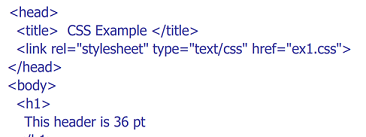
\includegraphics[scale=.8]{images/4.PNG}
\end{center}
\subsection{Recap sulla gerarchia delle classi}
\begin{center}
	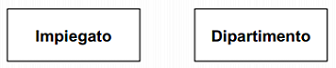
\includegraphics[scale=.8]{images/5.PNG}
\end{center}
\begin{itemize}
	\item La gerarchia si costruisce usando ciò che sappiamo con certezza (P contenuto in PSPACE) e le varie congetture.
	\item L’insieme più vasto è quello dei problemi decidibili.
	\item Abbiamo EXPTIME, all’interno del quale è presente PSPACE.
	\item All’interno di NP abbiamo P ed NP-completo. Un esempio di problema che non è P, ma neanche NP-completo, è la fattorizzazione (problema che ci interessa per la Crittografia). Questa cosa non è a caso: sulla macchina quantistica il problema è facilmente risolvibile.
\end{itemize}
Inoltre
\begin{itemize}
\item La classe P contiene problemi risolvibili in tempo polinomiale.
\item La classe NP contiene i problemi verificabili in tempo polinomiale (remember, verificare significa ottenere un certificato che attesta l'esistenza di una soluzione rispetto a una particolare istanza $I$)
\item I problemi NP-hard sono problemi a cui è possibile applicare il concetto di riduzione polinomiale: tutti i problemi appartenenti alla classe NP possono essere ridotti al problema NP-hard.
\item La classe NP-completo include tutti i problemi che appartengono ad NP e sono NP-hard. Se io risolvo uno di questi problemi risolvo tutti i problemi. Per verificare la possibilità di ridurre tutti i problemi di NP a un particolare problema uso il teorema di Cook, che afferma che qualsiasi problema NP si riduce a SAT: quindi se io posso ridurre SAT al problema in studio allora tutti i problemi NP possono essere ridotti al problema in studio.
\item Dato un problema posso definire il complementare, che accetta tutte le istanze rifiutate dal problema iniziale. Questo secondo problema appartiene alla classe co-P, ma anche a P. I problemi che appartengono ad NP appartengono anche a co-NP: si congettura che P $\neq$ co-NP (dato il certificato del problema iniziale non riesco a costruire automaticamente il certificato del problema complementato).
\end{itemize} 
